% Four-page NeurIPS-style workshop draft for TS4H advice.
\documentclass{article}

\PassOptionsToPackage{numbers,compress}{natbib}
\usepackage[dblblindworkshop]{neurips_2026}
\workshoptitle{Learning from Time Series for Health}

\usepackage[utf8]{inputenc}
\usepackage[T1]{fontenc}
\usepackage{hyperref}
\usepackage{xurl}
\usepackage{booktabs}
\usepackage{amsmath,amssymb,amsfonts}
\usepackage{graphicx}
\usepackage{microtype}

\graphicspath{{figures/}{figures/generated/}}

\title{Boundary Density Likelihood for Health Time-Series Event Detection}
\author{Anonymous Authors}

\newcommand{\xseq}{x_{1:T}}
\newcommand{\rate}{\lambda}
\newcommand{\kernel}{\kappa}
\newcommand{\Rnonneg}{\mathbb{R}_{\ge 0}}

\begin{document}
\maketitle

\begin{abstract}
Health time-series systems are often evaluated by sparse temporal detections:
sleep onset, wake-up, seizure boundaries, alarms, or episode endpoints.
Training dense state masks is an indirect surrogate when the benchmark later
matches ranked event times.
We propose Boundary Density Likelihood (BDL), a maximum-likelihood objective
that converts annotations into expected boundary counts per output bin and fits
nonnegative rates with a Poisson log score.
Unit-sum smoothing represents annotation uncertainty without changing the event
count.
Across sleep-event and CHB-MIT seizure benchmarks, BDL improves event mean
average precision under matched folds, architectures, and decoders.
On sleep, it improves GRU event mAP from 0.575 to 0.680 over cross-entropy
segmentation, with the largest gains at one- and three-minute tolerances.
The result should be read narrowly: BDL targets event AP, while direct
segmentation remains the right objective for samplewise occupancy.
\end{abstract}

\section{Motivation}

Long health recordings are commonly judged by a small set of times.
For sleep monitoring, an overnight interval is scored through onset and
wake-up matches; for seizure review, clinical utility depends on episode
boundary timing \citep{shoeb2010,goldberger2000,alexander2017,esper2023}.
Detection benchmarks therefore sort candidate times by confidence, match them
inside task-specific tolerance windows, and summarize precision--recall
\citep{everingham2010pascal,lin2014coco,salles2023}.
Samplewise accuracy can look strong while event AP is weak, because duplicated,
late, early, or poorly ranked boundaries are what the scorer consumes
\citep{tatbul2018precision}.

The usual reduction expands sparse annotations into dense state labels.
That is appropriate when deployment needs calibrated labels at every sample.
It is less direct when the downstream interface is a ranked onset, offset, or
alarm time.
Related areas already use localized supervision for keypoints, sound events,
action boundaries, and temporal proposals
\citep{newell2016stacked,xiao2018simple,phan2015,gao2017turn,lin2018bsn,lin2019bmn}.
The issue for health time series is what such a target means after smoothing,
clipping, and downsampling.
BDL gives it a count-preserving interpretation: each annotation contributes
one expected event, and the model estimates expected scored events per output
bin.

\section{Boundary Density Likelihood}

Let $\xseq$ be a time series and let $c$ index a scored event type.
For interval labels, onset and offset are represented as separate event types.
The annotations define a counting measure
\begin{align}
  \mu_c = \sum_{\tau\in B_c}\delta_\tau,
\end{align}
where $B_c$ is the set of type-$c$ boundary times.
We use point-process notation only to define the supervised target; BDL is not
a full event-history model \citep{kingman1993,shchur2021neural}.

To represent timing uncertainty, each point can be replaced by a nonnegative
kernel $\kernel$ with unit mass:
\begin{align}
  y_c(t) = \sum_{\tau\in B_c}\kernel(t-\tau), \qquad
  \sum_r \kernel(r)=1.
  \label{eq:smooth}
\end{align}
We use hard, truncated Gaussian, and tolerance-aligned kernels.
Because the kernel sums to one, smoothing changes where an annotation can
appear but not how many events it represents.
If output bin $b$ covers raw timesteps $G_b$, the binned target is the
integrated count
\begin{align}
  Y_c(b) = \sum_{t\in G_b} y_c(t).
  \label{eq:bin}
\end{align}
Thus downsampling sums expected events into coarser bins instead of averaging
away the target scale.

A sequence model emits logits $z_{\theta,c}(b)$, converted to nonnegative
rates $\rate_{\theta,c}(b\mid\xseq)$ by softplus with a sparse-event prior
initialization.
For one bin, the Poisson negative log score is
\begin{align}
  \ell(Y,\rate)=\rate - Y\log \rate,
\end{align}
omitting target-only constants.
The empirical objective is
\begin{align}
  \mathcal{L}_{\mathrm{BDL}}(\theta)
  =
  \sum_c\sum_b
  \left[\rate_{\theta,c}(b\mid\xseq)
  -Y_c(b)\log \rate_{\theta,c}(b\mid\xseq)\right].
  \label{eq:loss}
\end{align}
Zero-event windows penalize predicted events, while repeated nearby events can
produce counts larger than one.
The conditional expected risk is minimized when the output equals the expected
number of scored events in each bin, so the sequence output has a fixed unit
rather than an arbitrary heatmap scale \citep{gneiting2007proper}.
At inference, local maxima become ranked detections.
For on--off states such as sleep and wake, alternation or duration constraints
belong in decoding; the likelihood estimates endpoints, not legal intervals.

\section{Experiments and Results}

We test whether aligning training with event AP improves localization under
matched detector choices.
The sleep benchmark contains wrist accelerometer recordings with sleep onset
and wake-up annotations \citep{alexander2017,migueles2019,robbins2019,esper2023}.
It stresses the segmentation reduction because the state interval is long but
the scoring tolerances are minute-scale.
CHB-MIT seizure detection tests a different signal modality with second-scale
endpoint tolerances \citep{shoeb2010,goldberger2000,klem1999}.

All methods are trained as sequence predictors and evaluated as event
detectors.
BDL ranks peaks in learned event-score sequences.
Segmentation baselines predict interval masks and derive event scores from
state transitions.
Within each comparison we hold splits, backbone, event scorer, and decoder
calibration fixed.
Sleep experiments compare BDL-Hard, BDL-Gaussian, and BDL-Tolerance against
cross-entropy, class-weighted cross-entropy, and focal segmentation
\citep{krawczyk2016,lin2017focal}.
Architecture controls repeat the strongest objectives with a bidirectional
GRU, a one-dimensional U-Net, and an attention-gated U-Net
\citep{ronneberger2015,oktay2018attention}.

\begin{figure}[t]
\centering
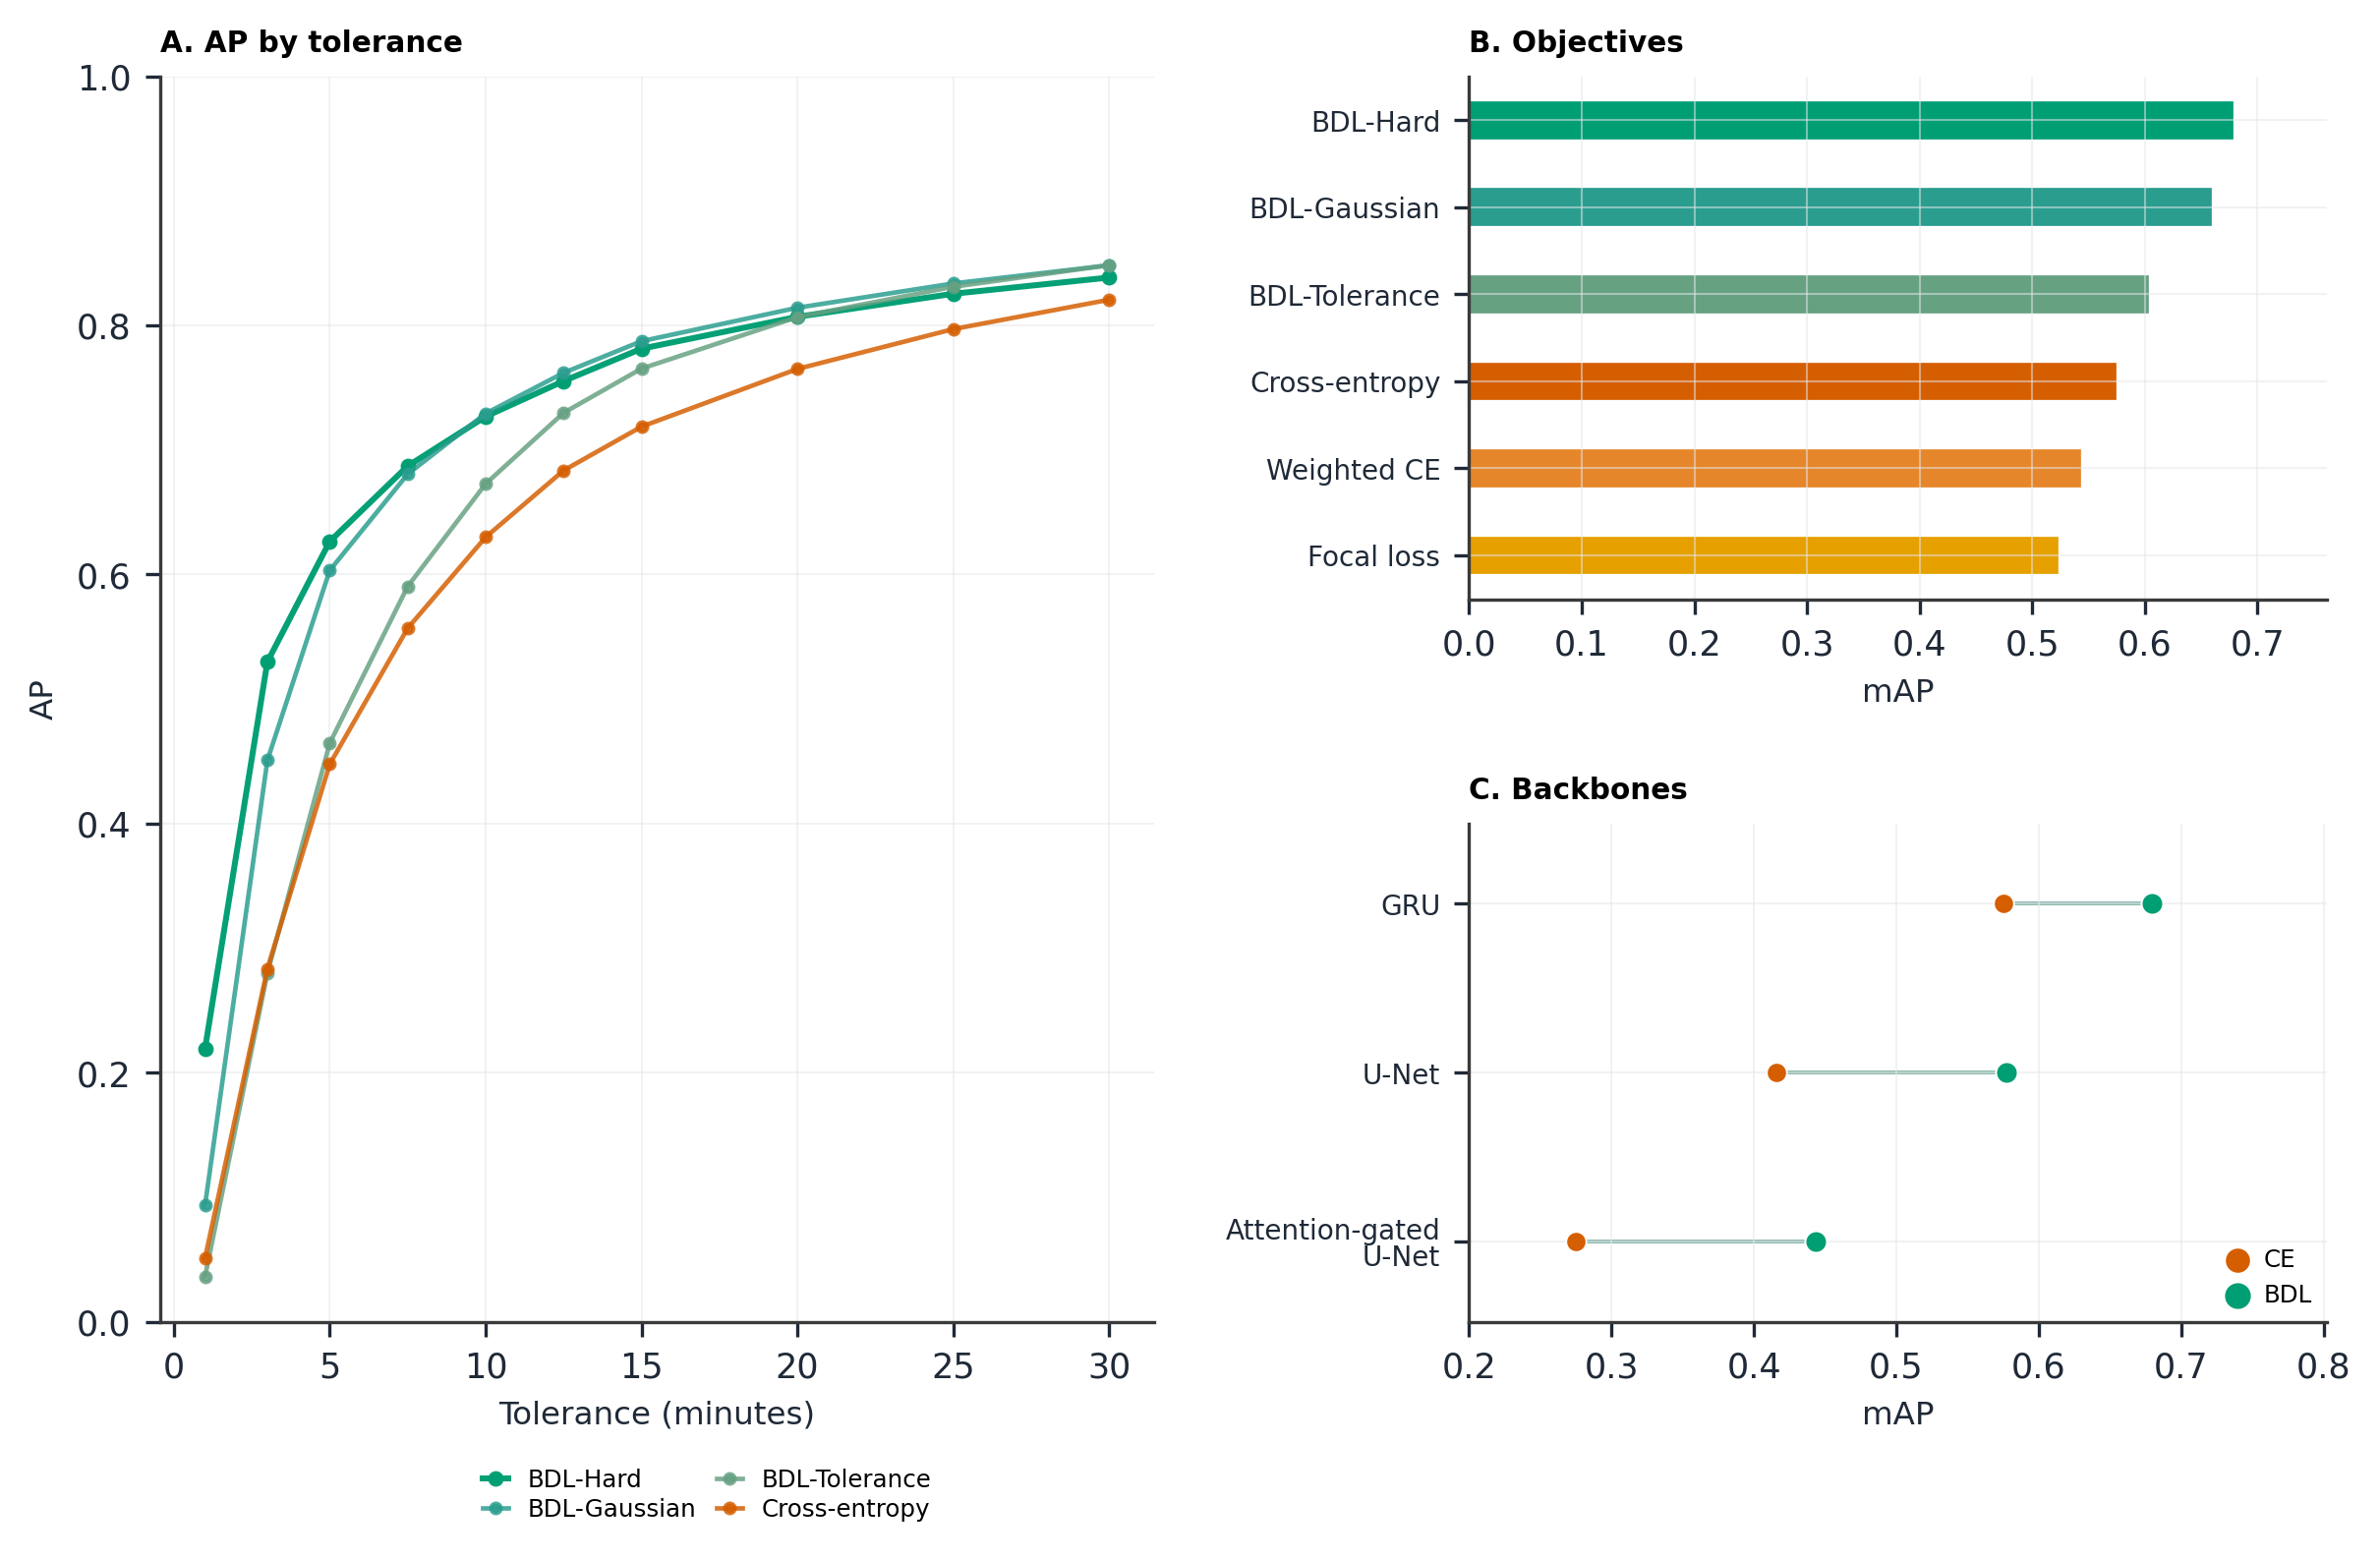
\includegraphics[width=0.98\linewidth]{sleep_main_results.png}
\caption{Sleep-event results under matched folds and event scoring.
BDL's advantage is largest at strict tolerances (A), remains above
segmentation losses in the objective sweep (B), and persists across recurrent
and convolutional backbones (C).}
\label{fig:sleep}
\end{figure}

Figure~\ref{fig:sleep} shows the central sleep result.
With the GRU fixed, BDL-Hard reaches 0.680 mAP, compared with 0.575 for
cross-entropy segmentation, 0.544 for class-weighted cross-entropy, and 0.525
for focal loss.
The difference is concentrated where timing is strict: one-minute AP improves
from 0.051 to 0.219, and three-minute AP from 0.283 to 0.530.
At thirty minutes the curves nearly meet, 0.821 versus 0.838, suggesting that
both methods often find the sleep episode, while BDL better ranks localized
endpoints.
BDL-Gaussian and BDL-Tolerance reach 0.660 and 0.605 mAP, so smoothing alone
does not explain the gain.

\begin{table}[t]
\centering
\small
\begin{tabular}{lccc}
\toprule
Setting & BDL & Seg. & $\Delta$ \\
\midrule
Sleep GRU & 0.680 & 0.575 & +0.104 \\
Sleep U-Net & 0.578 & 0.416 & +0.162 \\
Sleep attn. U-Net & 0.444 & 0.275 & +0.168 \\
CHB-MIT, 2 s stride & 0.360 & 0.252 & +0.108 \\
CHB-MIT, 1 s stride & 0.388 & 0.287 & +0.101 \\
\bottomrule
\end{tabular}
\caption{Compact event-mAP summary.  Each row compares matched folds,
architecture, scorer, and decoder calibration.}
\label{tab:summary}
\end{table}

Table~\ref{tab:summary} summarizes the broader evidence.
BDL-Hard remains above segmentation for the GRU, U-Net, and attention-gated
U-Net.
On CHB-MIT, the strongest BDL kernel changes with output stride, but the
matched comparison is stable: BDL-Gaussian improves two-second-stride mAP from
0.252 to 0.360, and BDL-Hard improves one-second-stride mAP from 0.287 to
0.388.
Strict one-to-three-second endpoint analysis preserves the direction for
BDL-Hard and BDL-Gaussian, although the tolerance-shaped kernel no longer
helps.

\begin{figure}[t]
\centering
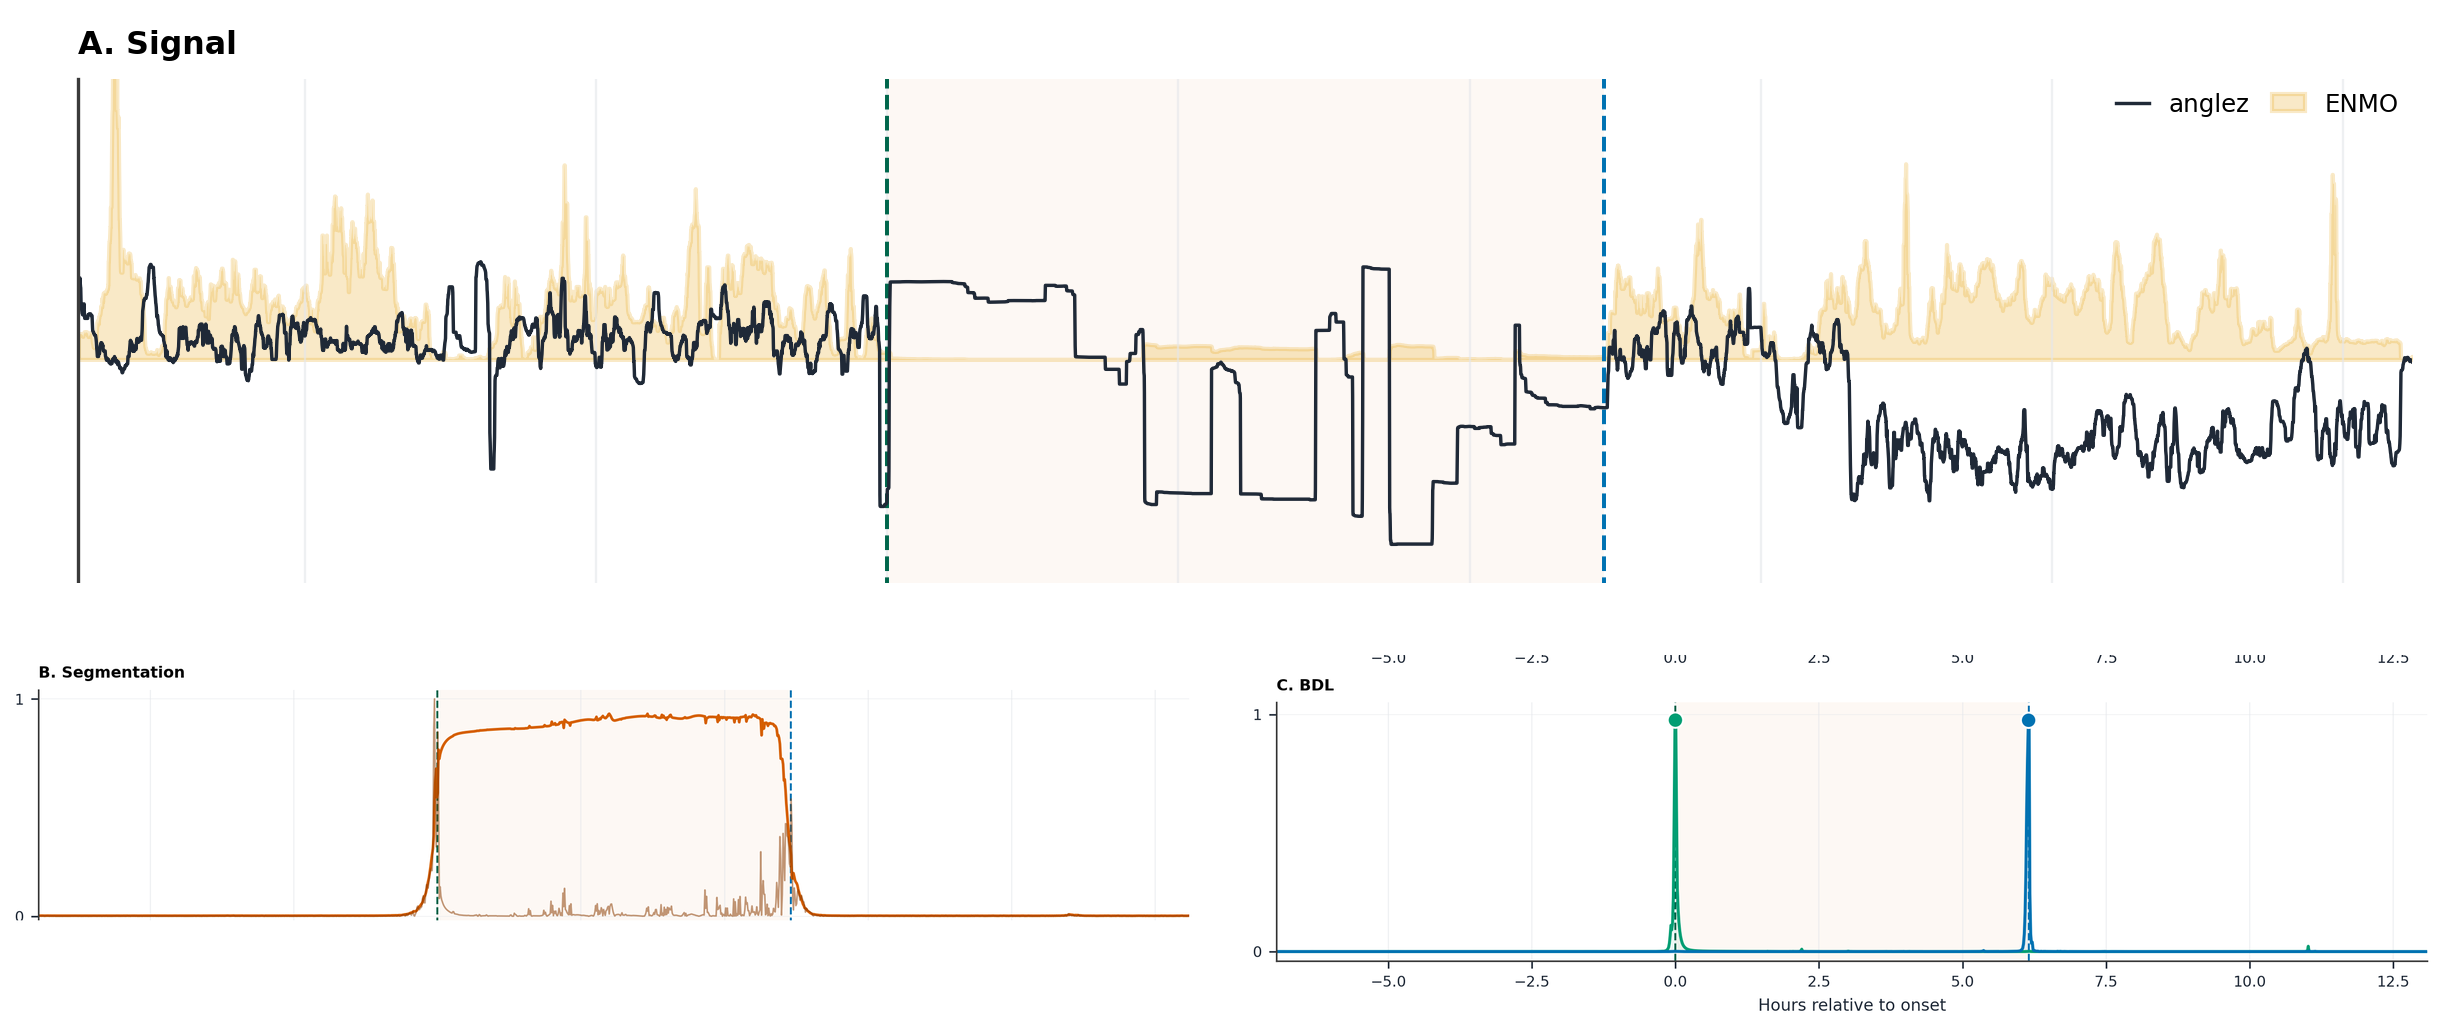
\includegraphics[width=0.98\linewidth]{sleep_prediction_compact.png}
\caption{Held-out sleep window.  Segmentation predicts a state interval and
derives boundary scores afterward; BDL directly scores the onset and wake-up
events matched by event AP.}
\label{fig:qualitative}
\end{figure}

\section{Related Work and Scope}

BDL is closest in spirit to heatmap or proximity supervision, but its output
has a different unit.
In keypoint, sound-event, and action-boundary work, localized heatmaps are
often useful engineering labels; in health recordings, however, kernel width,
window clipping, and output stride can silently change the target mass.
Equations~\eqref{eq:smooth}--\eqref{eq:loss} keep the unit fixed as expected
scored events per bin.
This matters for long empty windows, repeated events, and multi-resolution
training, where an arbitrary dense scale can change the false-positive
pressure seen by the model.

The state-reconstruction diagnostic makes the scope explicit.
When predictions are converted back to sleep-state intervals and scored by
samplewise F1, direct cross-entropy segmentation remains stronger than BDL
hazard reconstruction, 0.914 versus 0.888.
This is not a contradiction: BDL changes what the sequence output estimates
when the benchmark matches ranked event times, while state labels remain the
direct target for samplewise occupancy.

BDL is also more modest than a temporal point process.
It does not model censoring, mark dynamics, or clinical event generation.
Its contribution is to give heatmap-style boundary supervision a likelihood
and a unit: expected scored events per output bin.
That separation is useful in health deployments.
If the deployed system needs legal sleep intervals, alternating onset/offset
pairs, or duration priors, those constraints should be decoded and evaluated
explicitly rather than hidden inside a segmentation surrogate.

\section{Conclusion}

Boundary Density Likelihood addresses a common mismatch in health time-series
detection: models are often trained as samplewise segmenters but evaluated by
ranked event times.
By fitting expected boundary counts with a Poisson log score, BDL keeps the
practical advantages of sequence prediction while making the output estimate
the temporal detections that event metrics later match.
The current results support BDL as a simple objective-level fix for event AP,
with segmentation retained as the appropriate baseline when the target is
samplewise state estimation.

Two limitations are important for the workshop version.
First, likelihood alignment does not remove decoder design.
Endpoint pairing, alternating onset/offset constraints, refractory windows,
and duration priors should be applied after scoring and ablated separately,
especially for on--off processes such as sleep.
Second, event gains should be reported alongside state reconstruction whenever
the same detections might be used to recover intervals.
That paired view is what keeps the claim honest: BDL is not a universal
replacement for segmentation, but a likelihood-based target for detectors whose
primary output is a ranked temporal event.

\clearpage
\bibliographystyle{plainnat}
\bibliography{main}

\end{document}
